%!TEX root = Thesis_David_Burns.tex
\chapter{Methodology}
\label{ch:meth}

%--------------------------------------------------------------------------------------------------------------------------%
%--------------------------------------------------------------------------------------------------------------------------%

\section{Models}
\label{sec:ccg}

	The first part of this project involves modelling the source of air at particular locations. For this \gls{hysplit} was used as it is an established back trajectory model (see \cref{sec:backtraj}). The three models used in the second part of this project were \gls{ccam}, \gls{ctm} and \gls{glomapm} (see \cref{sec:ccg}). \gls{ccam} provides the meteorological data needed for \gls{ctm} and \gls{ctm} provides the chemical concentration data required for \gls{glomapm}. However, currently the system is limited to running \gls{ccam} offline from the other models (see \cref{fig:modelstruct}) \citep{mcgregor2008updated}. Thus there is no feedback into the meteorology from changes in chemical or aerosol levels, such as cloud production caused by changes in \gls{ccn} concentrations.

	\begin{figure}[!htb]
	    \centering
	    \vspace*{5mm}
	    \includegraphics[width=0.8\textwidth]{Fig/Research/ModelStructure.tikz}
	    \vspace*{5mm}
	    \caption{The group of models prepared by \gls{csiro} for modelling from meteorology to aerosols. Arrows indicate the direction data passes.}
	    \label{fig:modelstruct}
	\end{figure}

%--------------------------------------------------------------------------------------------------------------------------%

	\subsection{HYSPLIT}
	\label{subsec:hysplit}

	\gls{hysplit} is the Hybrid Single Particle Lagrangian Integrated Trajectory model developed by the National Oceanic and Atmospheric Administration and Australia's Bureau of Meteorology. It takes as input a variety of different meteorological data sources to produce the field the parcel of air being tracked travels through.

	A Lagrangian model may be implemented in two different ways. A puff model regularly releases and follows a parcel of air containing the required fraction of trace components. The puff moves and expands depending on advection and diffusion respectively. A particle model releases many single particles which are moved through advection, but which are also randomly moved based on the diffusion present \citep{draxler:1997tga}. \gls{hysplit} implements a hybridisation of these models by using the particle style for vertical motion, and the puff style for horizontal motion \citep{hurley:1994df}.

	The user provides a location and time for the start of the trajectory, and the amount of time backwards or forwards for it to run. \gls{hysplit} produces a line of latitude and longitude points where each point is an amount of time away from the starting time. Thus the line through the points indicates the trajectory, backwards or forwards through time of the air at the starting location.

	\gls{hysplit}, like all atmospheric models, is sensitive to initial conditions \citep{challa2008sensitivity} and its accuracy is dependent on the error margins of the meteorological data it makes use of \citep{draxler:1998vr}. The results of any trajectory run are therefore less accurate the further away from the initial conditions the trajectory gets. There is also a dependence on the spatial and temporal granularity of the meteorological data. As such, \gls{hysplit} offers the ability to slightly permute the initial conditions of the model to produce a multitude of possible trajectories for a single location and time \citep{draxler:1997tga}. It is also possible to produce multiple trajectories over time or over space and a robust scripting platform exists to allow this \citep{draxler:1997tga}.

	\subsubsection{\gls{hysplit} Visualisations}
	\label{subsubsec:hysvis}

	A technique for producing meaningful visualisations of this modelling system, given it's shortcomings, is to produce a normalised histogram of multiple trajectories. The GUI side of \gls{hysplit} offers a method for doing this using the bulk production of trajectories from permuted initial conditions \citep{draxler:1997tga}.  A spatial domain is subdivided into boxes, then whatever points of the various trajectories that lie in that box are counted. Each box is then normalised by the total number of trajectory points in the domain. It is then possible to plot these boxes onto a map of the region, colouring them based on their values. This technique provides a visual idea of whether a given parcel of air will have passed over that box. Similarly, by producing multiple trajectories over time, it is possible to create a visualisation of the likelihood that a parcel of air has passed through a box within a time period.
	
	If the number of points in box $i$ is $N_i$ then the fraction of the total points being in that box $f_i$ is given by,
	\begin{align}
		f_i = \frac{N_i}{\sum_{i=1}^m N_i},
	\end{align}
	where $m$ is the total number of boxes \citep[Chapter 3]{lefebvre:2006vi}.

	Another visualisation tool is to create a time series of the trajectories, overlaid on a map, in a movie. This shows how the trajectory evolves with the changing meteorological conditions. This could be coupled with the interpolated histograms computed using small variations of the initial conditions to produce a better idea of probable trajectories' evolution through time.

	\subsection{CCAM}
	\label{subsec:ccam}

	\gls{ccam} is \gls{csiro}'s Conformal-Cubic Atmospheric Model. Most \gls{rcm}s are performed on a grid that simulates only the area of interest, requiring spatial boundary conditions to be fed into the model at each time step \citep{hurley2002air}. Because of \gls{ccam}'s approach of conformal cubic mapping, the majority of grid points can be focussed onto the region of interest while still simulating the rest of the globe with a gradient of accuracy (see \cref{fig:ccammap}). This removes the necessity for boundary conditions as the full globe is being simulated, which allows distant events to influence the region of interest. However, there are fewer grid points in distant regions, sacrificing accuracy for computation time \citep{mcgregor:2005wz}.

	\begin{figure}[!htb]
    	\centering	    
		\begin{subfigure}[b]{0.8\textwidth}
			\centering
    		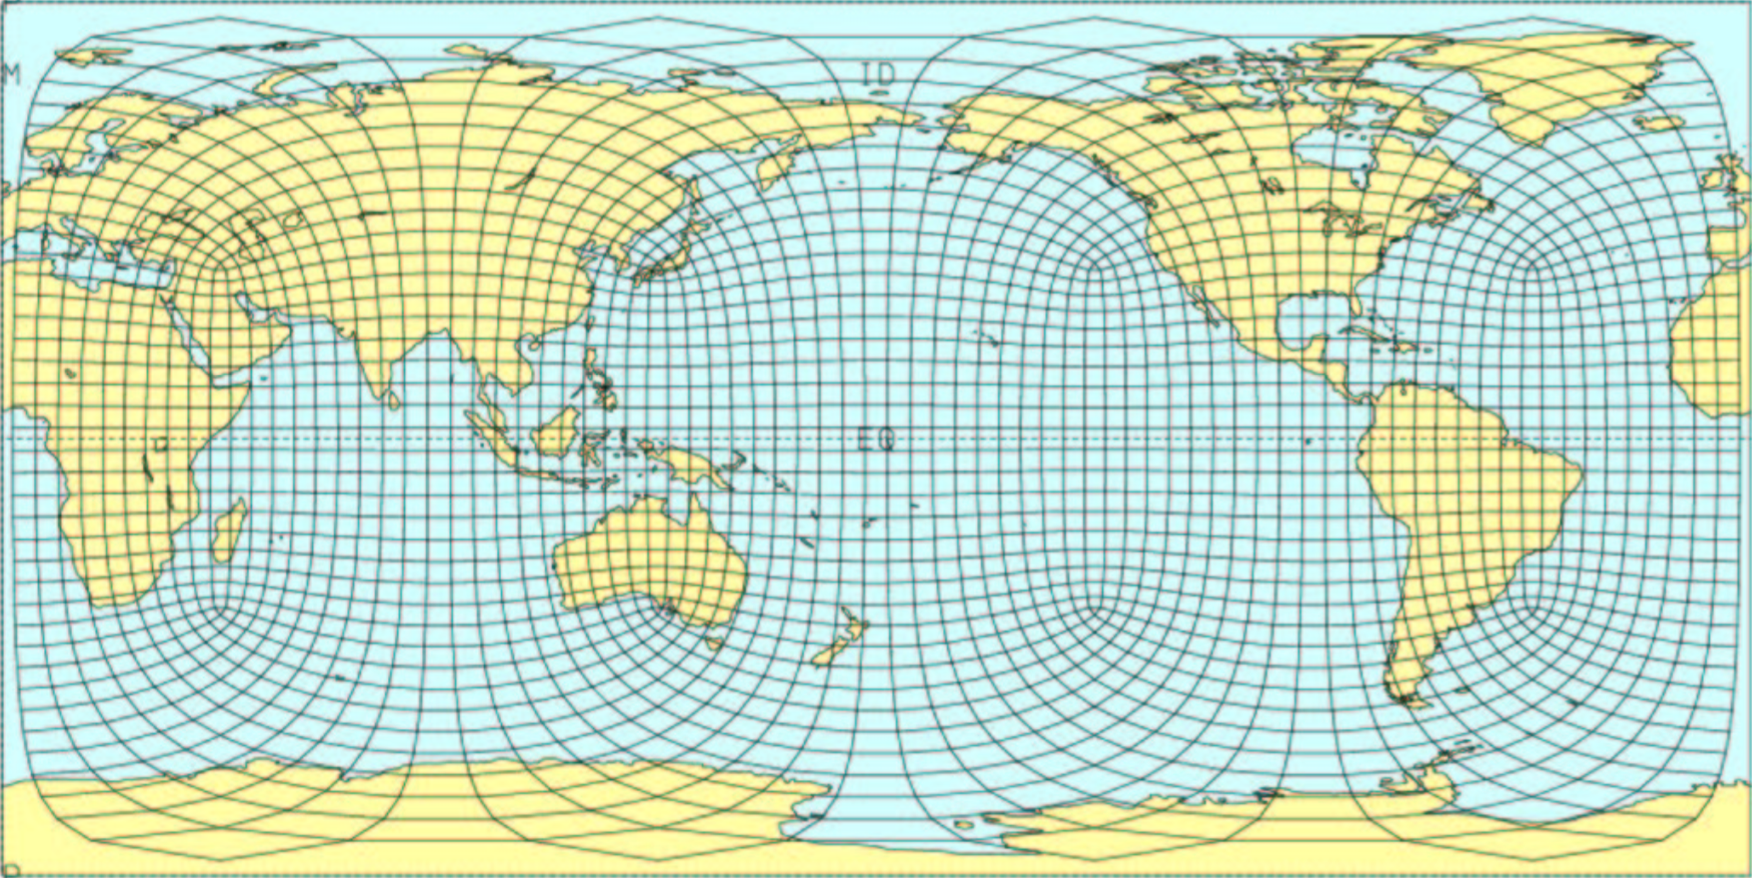
\includegraphics[width=\textwidth,natwidth=1752,natheight=878]{Fig/Research/ccamnormal.png}
			\caption{Unfocused Transformation}
			\label{fig:ccammapnorm} 
		\end{subfigure}

		\begin{subfigure}[b]{0.8\textwidth}
		\centering
    		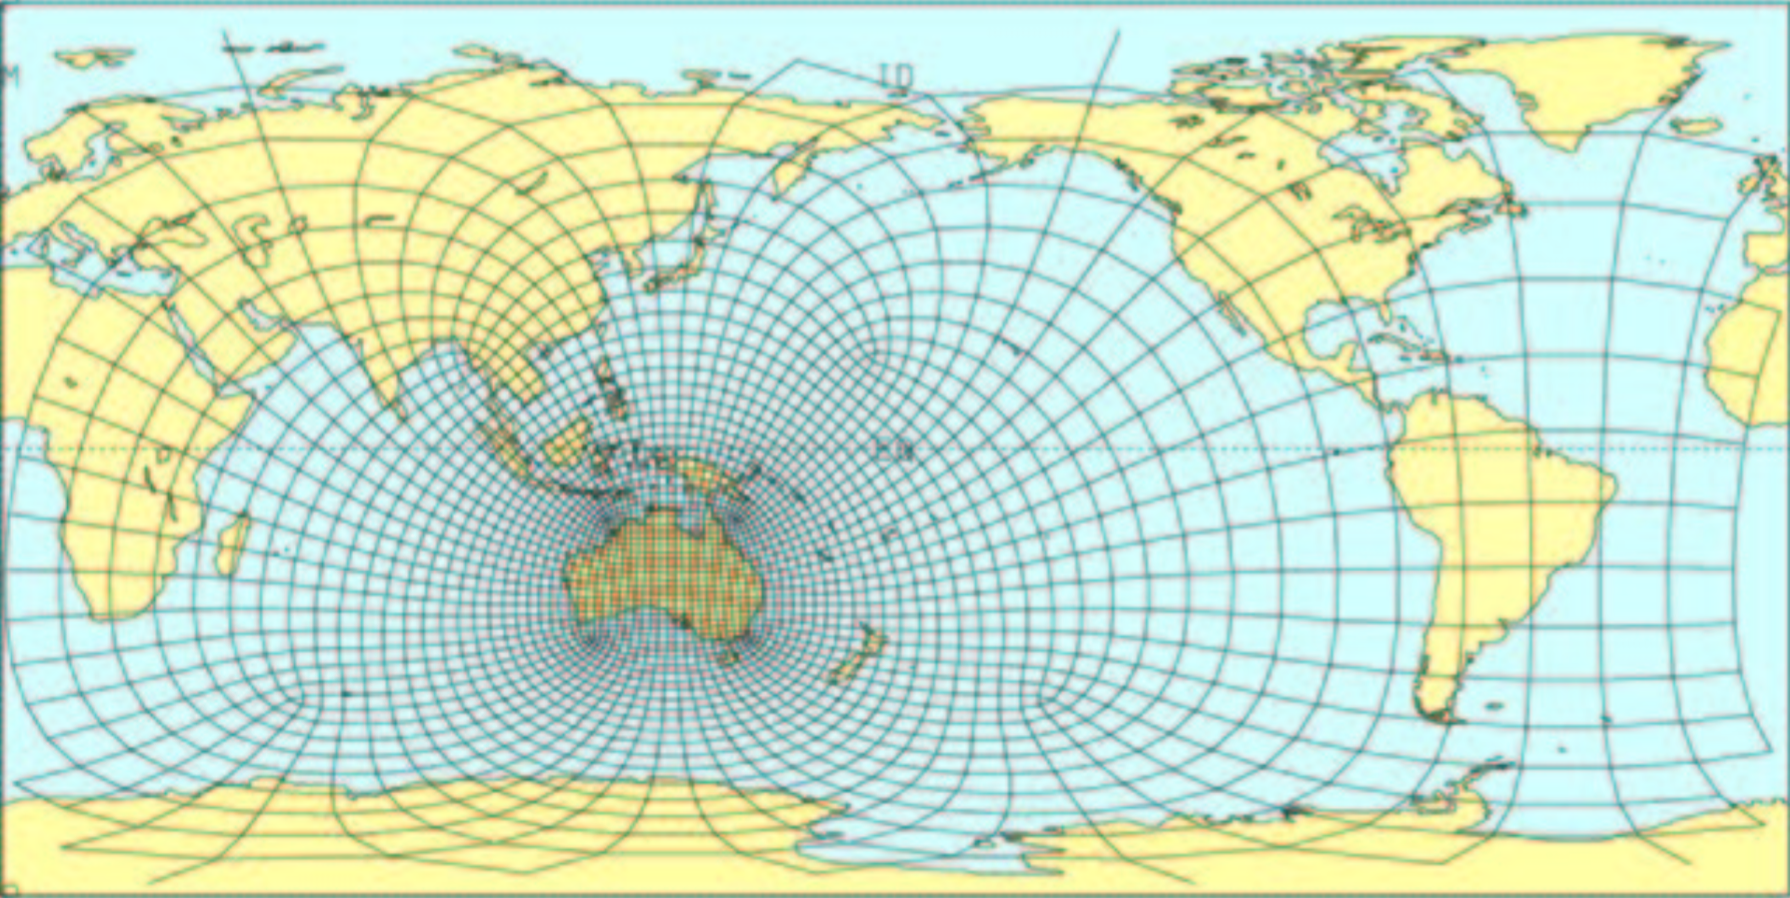
\includegraphics[width=\textwidth,natwidth=1790,natheight=898]{Fig/Research/ccamfocussed.png}
			\caption{Focused Transformation}
			\label{fig:ccammapfocus}
		\end{subfigure}

		\caption{Two examples of the conformal cubic mapping, used by \gls{ccam}, showing both a focussed and unfocussed transformation of the grid \citep{mcgregor:2005wz}. The focused transformation has a lower Schmidt number than the unfocussed transformation.}
    	\label{fig:ccammap}
	\end{figure}

	As inputs \gls{ccam} can accept data sets from a \gls{gcm} and nudge the model towards these values \citep{mcgregor:2005wz}. Although work is being done to incorporate a coupled ocean model with matching grid structures, without this the oceanic parameters, such as sea surface temperature, must be input as both spatially and temporally varying maps \citep{mcgregor2008updated}. Despite the non-uniformity of the cubic grid structure, \gls{ccam} produces latitude and longitude based output through interpolation of the cubic grid data \citep{thatcher:2015wy}.

	The current implementation of \gls{ccam} uses a semi-Lagrangian solver that is semi-implicit and non-hydrostatic, programmed in FORTAN. The solver is designed for expansion to a large number of cores, while dealing with the singularity-like points caused by the cubic mapping \citep{thatcher:2015wy}. It is also possible to run the model multiple times, focussing the grid in at each step while nudging is performed using the previous runs' data \citep{mcgregor2008updated}.

	Due to the nature of the grid structure \gls{ccam} uses, any domain must be transformed to match the inputs \gls{ccam} uses. These inputs are the latitude and longitude of the domain's centre, the grid size, and the Schmidt number. The grid size is the number of grid squares horizontally or vertically, as the domain must be square. The Schmidt number scales the front panel of the cube that approximates the globe. So the centre point positions the front face of the cube, the Schmidt number scales the face, and the grid size defines the resolution. 

	The Schmidt number $S$ is calculated from the length of the domain in degrees $L_d$, 
	\begin{align}
		\label{eq:schmidtnum}
		S &= \frac{L_d}{90}.
	\end{align}
	The grid size $g$ is calculated through the length of the domain in kilometres $L_k$ and the resolution, or length of an individual grid square in kilometres $R_k$,
	\begin{align}
		\label{eq:schmidtnum}
		g &= \frac{L_k}{R_k}.
	\end{align}

	The grid size chosen greatly effects the parallelisation of the model and thus the runtime \citep{thatcher:2015wy}. It is best to try and find the closest acceptable grid size, and then modify the Schmidt number to maintain the desired resolution, without changing the size of the domain too much.


%--------------------------------------------------------------------------------------------------------------------------%

	\subsection{CTM}
	\label{subsec:ctm}

	\gls{ctm} is the Chemical Transport Model produced at \gls{csiro}. It deals with various transport processes relating to chemicals found in the atmosphere, as well as deposition onto particles, changes in chemical structure, and emission sources \citep{cope:2009tz}. It uses a regular grid structure which requires boundary conditions (see \cref{fig:sydpartgrid}) that are usually taken from a \gls{gcm} \citep{cope:2014tw}. The transport of each chemical species is modelled using an advection diffusion equation around the chemical's concentration, with source terms relating to different chemical processes. Each of these are themselves modelled and solved before being fed back into the advection diffusion solver \citep{cope:2009tz}. 

	\begin{figure}[!htb]
    	\centering
    	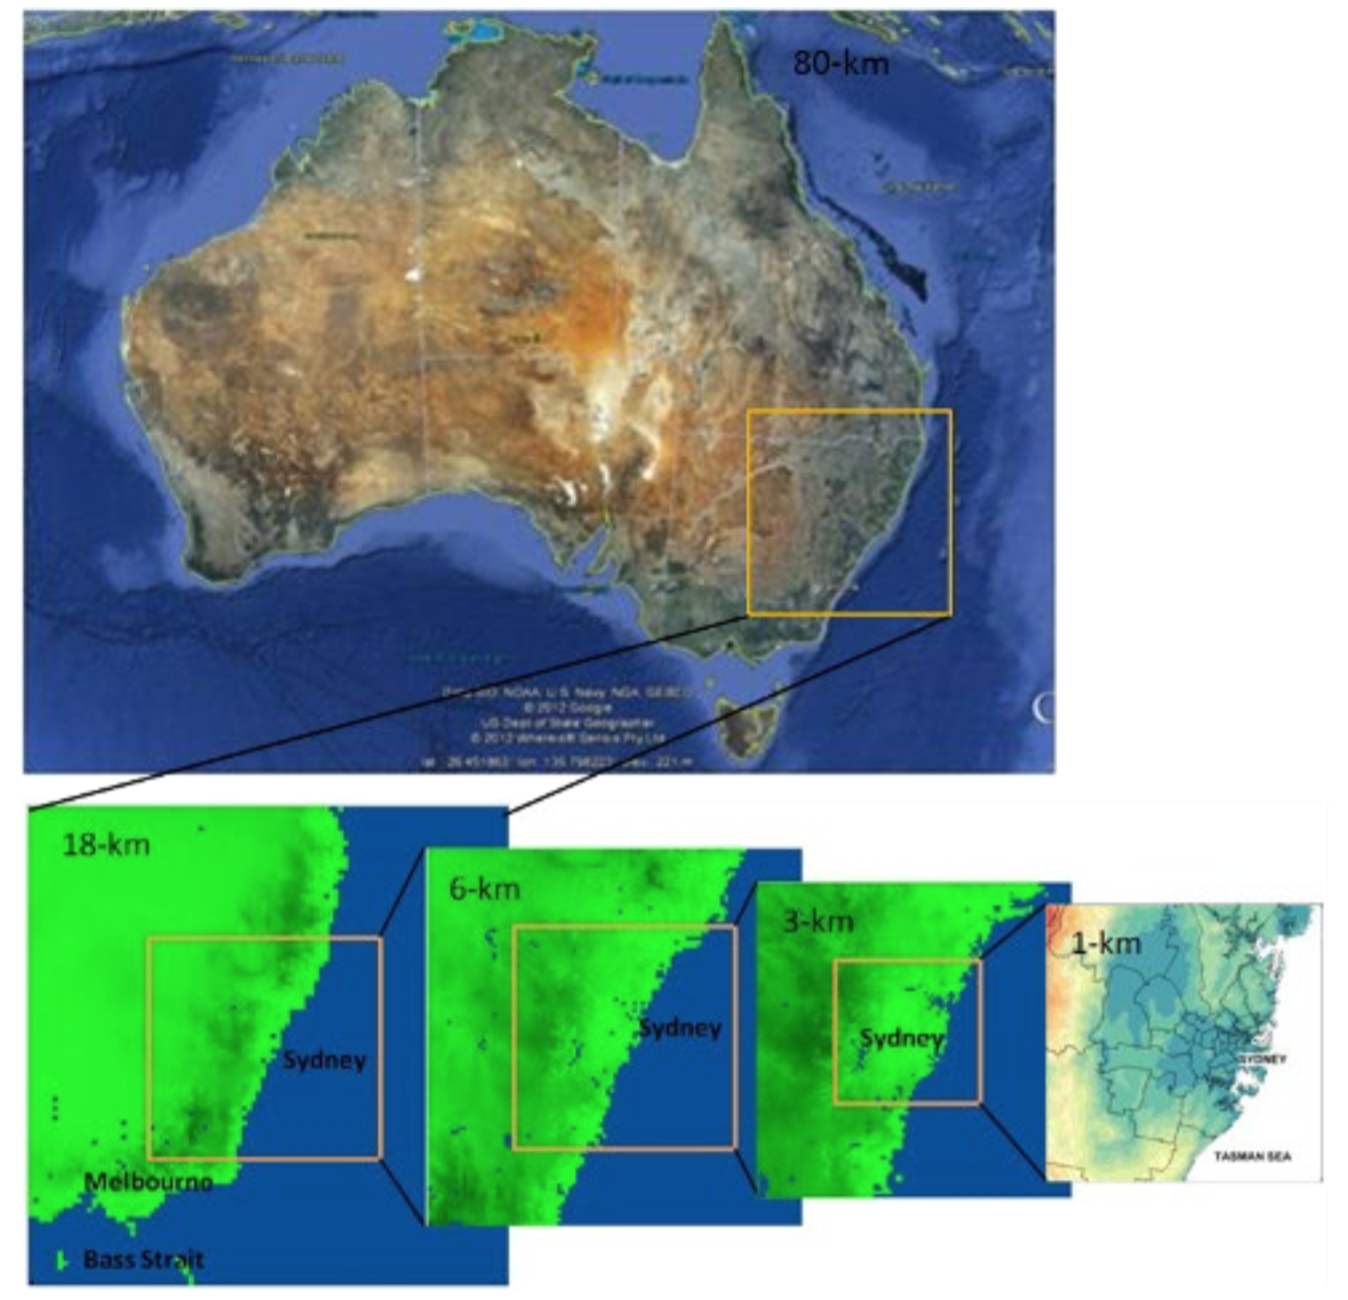
\includegraphics[width=0.8\textwidth,natwidth=1308,natheight=952]{Fig/Research/ctmexample.png}
    	\caption{A series of the zooming \gls{ctm} grids used in the Sydney Particle Study. An example of a \gls{ctm} produced chemical concentration map can be see at the bottom right \citep{cope:2014tw}.}
    	\label{fig:sydpartgrid}
	\end{figure}

	\gls{ctm} is written in FORTRAN, but allows for chemical reactions to be entered as regular form chemical equations \citep{cope:2009tz}. It requires a meteorological map as input, along with initial and boundary conditions for each chemical being tracked. Maps for the introduction of chemicals from the surface to the atmosphere are also required, such as when \gls{dms} is produced by the \gls{gbr}. \gls{ctm} outputs atmospheric maps of chemical concentrations.

	\gls{ctm} defines the domain through the latitude and longitude of the bottom left grid point $(BL_{Lat}, BL_{Lon})$, the number of horizontal and vertical grid points $(n_x, n_y)$, and the horizontal and vertical distance between grid points $(d_x, d_y)$.
	Taking a square domain defined via its centre point $(C_{Lat}, C_{Lon})$, its width and resolution in degrees $L_d, R_d$, then,
	\begin{align}
		\label{eq:dxdy}
		d_x = d_y &= R_d.
	\end{align}
	So,
	\begin{align}
		\label{eq:nxny}
		n_x = n_y &= \frac{L_d}{d_x}.
	\end{align}
	Thus,
	\begin{align}
		\label{eq:bottomleft}
		(BL_{Lat}, BL_{Lon}) &= (C_{Lat}, C_{Lon}) - \frac{n_x d_x}{2}.
	\end{align}

%--------------------------------------------------------------------------------------------------------------------------%

	\subsection{GLOMAP and GLOMAP-mode}
	\label{subsec:glomap}

	\gls{glomap} is the aerosol micro-physics component of the \gls{ukca} model developed at Leeds university. It uses atmospheric information and chemical concentrations to simulate the large amount of interactions aerosols undergo. It models new particle formation, condensation, cloud processing, hygroscopic growth and many other aerosol processes \citep{mann:2010wb}.

	\gls{glomapm} is an alternate version of \gls{glomap} which segregates aerosols via modes (see \cref{sec:aerosols}) rather than the \gls{glomap}'s direct bin approach. \gls{glomapm} also uses the equilibrium Henry's law style aqueous phase reactions recommended by \citet{barnes:2006ug}, while \gls{glomap} uses a more computationally expensive diffusion limited method \citep{mann:2010wb}. Both differences make \gls{glomapm} less accurate, but also less computationally expensive. Some treatments of particles are also adjusted to better make use of the modal structure. An example is that \gls{glomap} applies rain-out to any particles over \SI{103}{\nm}, while \gls{glomapm} applies rain-out to soluble particles in the accumulation and coarse modes \citep{mann:2010wb}. For modelling \gls{dms} and its aerosol products, \gls{glomap} uses the sulphur oxidation steps outlined in \citet{seinfeld2012atmospheric} and precomputed Henry's law coefficients \citep{mann:2010wb}. 

	The chemical concentration maps needed to feed into \gls{glomap} can either be offline, computed beforehand, or online \citep{mann:2010wb}. Online maps are updated by what is consumed or produced within \gls{glomap} and then passed to a chemical transport model running above \gls{glomap} \citep{spracklen2003development}. \gls{glomap} produces maps of aerosol concentrations, separated into bins or modes depending on the version used.

%--------------------------------------------------------------------------------------------------------------------------%
%--------------------------------------------------------------------------------------------------------------------------%

\section{Study Design}
\label{sec:std}

%Reminders:
%	- Reference your literature review as you are going
%	- Be specific about values you are using

The modelling work in this project is connected to a number of real world experiments to measure the \gls{gbr}'s effect on climate. This guided much of the design of the study. A number of land based research centres along the Queensland coast needed to be assessed for viability, to see if the majority of the air they received passed over the \gls{gbr}. A ship voyage was also planned off the coast of Queensland, providing a second series of locations to assess. Back trajectory modelling would be used to study the source of air at these experimental locations. It is important for the locations chosen to have minimal influence from land based aerosol sources as those sources will dominate \gls{dms} derived particles. The final chosen locations of the experimental work, directed by this back trajectory modelling, in turn established the position and size of the domains for the aerosol modelling.
 
\subsection{Assessing Locations}
\label{subsec:hyex}

The visualisation technique proposed in \cref{subsubsec:hysvis} was developed to examine the source of air at a location. HYSPLIT was used for modelling back trajectories. To produce the mass back trajectories needed for creating the histogram, a script was developed for running HYSPLIT a large number of times. Alongside this, visualisation scripts to produce the normalised histograms were created. 

A number of locations both on and off the coast of Queensland were selected (see \cref{tab:hysplitlocs}). Back trajectories were modelled at $4$ hourly intervals with each trajectory spanning back $120$ hours. Year long runs were performed first to gauge the best months. Four years were modelled, from $2011$ to $2014$. To produce the monthly plots the trajectories from all four years, for each month, were collected and processed to create histograms based on latitude and longitude. The histograms were interpolated and plotted over a map of Queensland.

\begin{table}[tbh!]
	\caption{\textsl{ The list of experimental coastal locations along the Queensland coastline that HYSPLIT was run for. }}
	\centering
		\begin{tabular}{c c c} \\
			\hline \\ [-1ex]
			Name & Latitude & Longitude \\ [1ex]
			\hline \\ [-1ex]
			Whitsundays & -20.06 & 148.95 \\
    		AIMS Cape Ferguson & -19.27 & 147.06 \\
    		Orpheus Island & -18.63 & 146.50 \\
			Lucinda Jetty & -18.52 & 146.39 \\
			Cairns & -16.88 & 145.94 \\
			TCU Daintree Forest Observatory & -16.10 & 145.44 \\
			Lizard Island & -14.67 & 145.45 \\ [1ex]
			\hline \\
		\end{tabular}
	\label{tab:hysplitlocscoast}
\end{table}

\begin{table}[tbh!]
	\caption{\textsl{ The list of experimental ship locations between the \gls{gbr} and \gls{qld} coastline that HYSPLIT was run for. }}
	\centering
		\begin{tabular}{c c c} \\
			\hline \\ [-1ex]
			Name & Latitude & Longitude \\ [1ex]
			\hline \\ [-1ex]
			Mackay & -21.12 & 149.71 \\
			Hamilton & -19.98 & 149.11 \\
			Townsville & -19.24 & 147.67 \\
			Great Palm Isl & -18.62 & 146.72 \\
			Innisfail & -17.53 & 146.23 \\
			Cape Tribulation & -16.09 & 145.56 \\ [1ex]
			\hline \\
		\end{tabular}
	\label{tab:hysplitlocsship}
\end{table}

\begin{figure}[!htb]
    \centering
    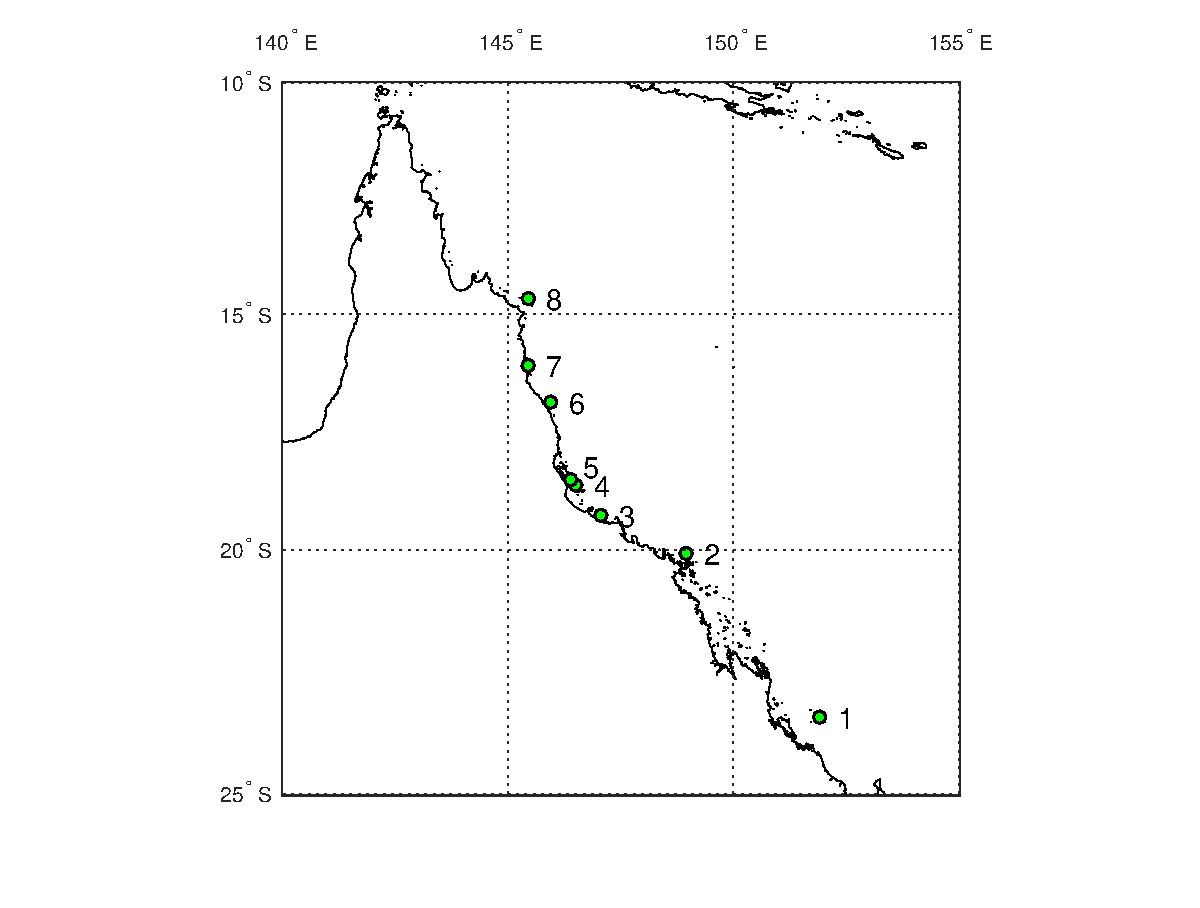
\includegraphics[width=0.9\textwidth]{Fig/Research/CoastLocs.eps}
    \caption{The series of coastal locations chosen for modelling back trajectories. }
    \label{fig:coastlocs}
\end{figure}

\begin{figure}[!htb]
    \centering
    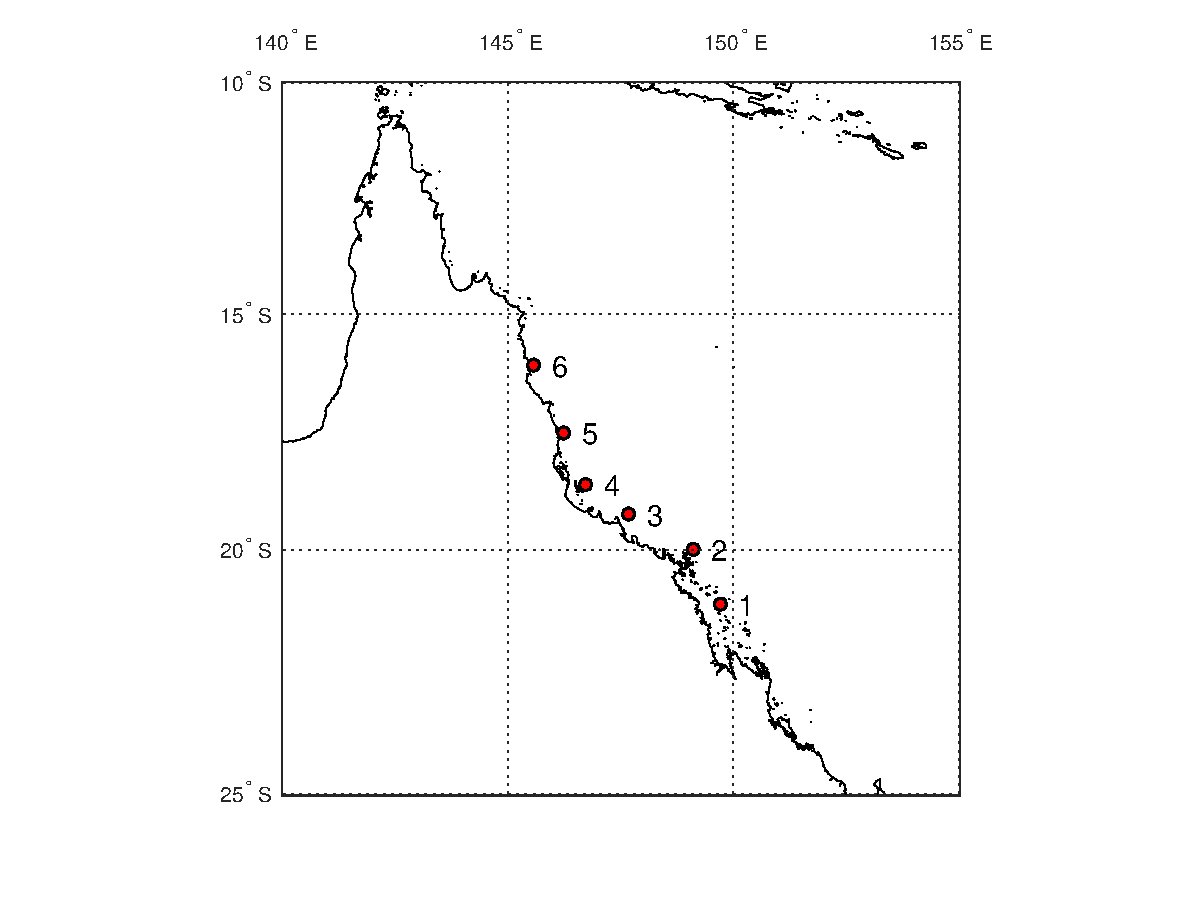
\includegraphics[width=0.9\textwidth]{Fig/Research/ShipLocs.eps}
    \caption{The series of ship based locations chosen for modelling back trajectories. }
    \label{fig:shiplocs}
\end{figure}

\subsection{CCAM and CTM Domains}
\label{subsec:domains}

As both \gls{ctm} and \gls{ccam} approach defining domains differently, a series of initial domains were chosen. The centre point was selected to be $-19.62$, $148.36$, latitude and longitude, using square domains with width \SIlist[list-units = single]{6000;2000;1000}{\km}, with resolutions of \SIlist[list-units = single]{80;9;3}{\km} respectively. The tiered domain structure, with decreasing width but increasing granularity, allows for greater detail at the coastal level. Distant effects, from inland Australia and out to the Pacific Ocean, are still simulated but with lower acuity. This approach attempts to ensure all the important influences are modelled without requiring exorbitant computation times.

Applying the equations in \cref{subsec:ccam} and \cref{subsec:ctm} produces the domains for each model. The \gls{ccam} domain was calculated first, and the \gls{ctm} domain was calculated from the \gls{ccam} domain after shrinking it by \SI{90}{\percent}. This was done to avoid the singularities at the corners of the \gls{ccam} domain.

\begin{table}[tbh!]
	\caption{\textsl{The values defining the domains used in \gls{ccam} for modelling the atmosphere over the Great Barrier Reef}}
	\centering
		\begin{tabular}{c c c c c} \\
			\hline \\ [-1ex]
			Name & Centre Latitude & Centre Longitude & Grid Size & Schmidt Number \\ [1ex]
			\hline \\ [-1ex]
			GBR 1 & -19.62 & 148.36 & 72 & 0.6 \\ 
 			GBR 2 & -19.62 & 148.36 & 288 & 0.2 \\
			GBR 3 & -19.62 & 148.36 & 384 & 0.1 \\ [1ex]
			\hline \\
		\end{tabular}
	\label{tab:ccamdomain}
\end{table}

\begin{table}[tbh!]
	\caption{\textsl{The values defining the domains used in \gls{ctm} for modelling the chemical transport and aerosol micro-physics over the Great Barrier Reef}}
	\centering
		\begin{tabular}{c c c c c} \\
			\hline \\ [-1ex]
			Name & Bottom Left & Bottom Left & Number of & Distance Between \\
			& Latitude & Longitude & Grid Points & Grid Points \\ [1ex]
			\hline \\ [-1ex]
			GBR 1 & -43.385 & 124.595 & 50 & 0.97 \\ 
 			GBR 2 & -27.62 & 140.36 & 81 & 0.2 \\
 			GBR 3 & -23.6325 & 144.3475 & 108 & 0.075 \\ [1ex]
			\hline \\
		\end{tabular}
	\label{tab:ctmdomain}
\end{table}

\begin{figure}[!htb]
    \centering
    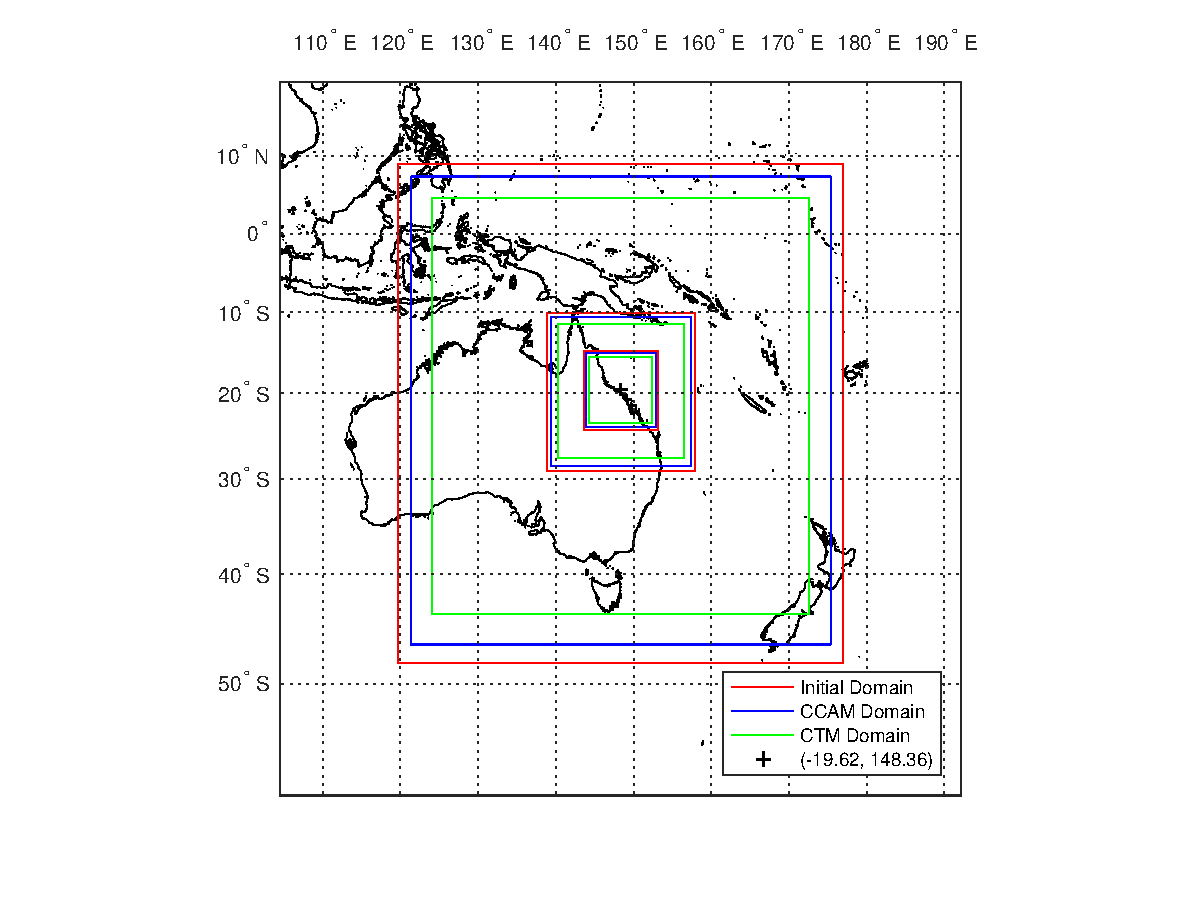
\includegraphics[width=0.9\textwidth]{Fig/Research/Domains.eps}
    \caption{A series of three tiered initial domains with their accompanying \gls{ccam} and \gls{ctm} domains.}
    \label{fig:domains}
\end{figure}

\begin{figure}[!htb]
    \centering
    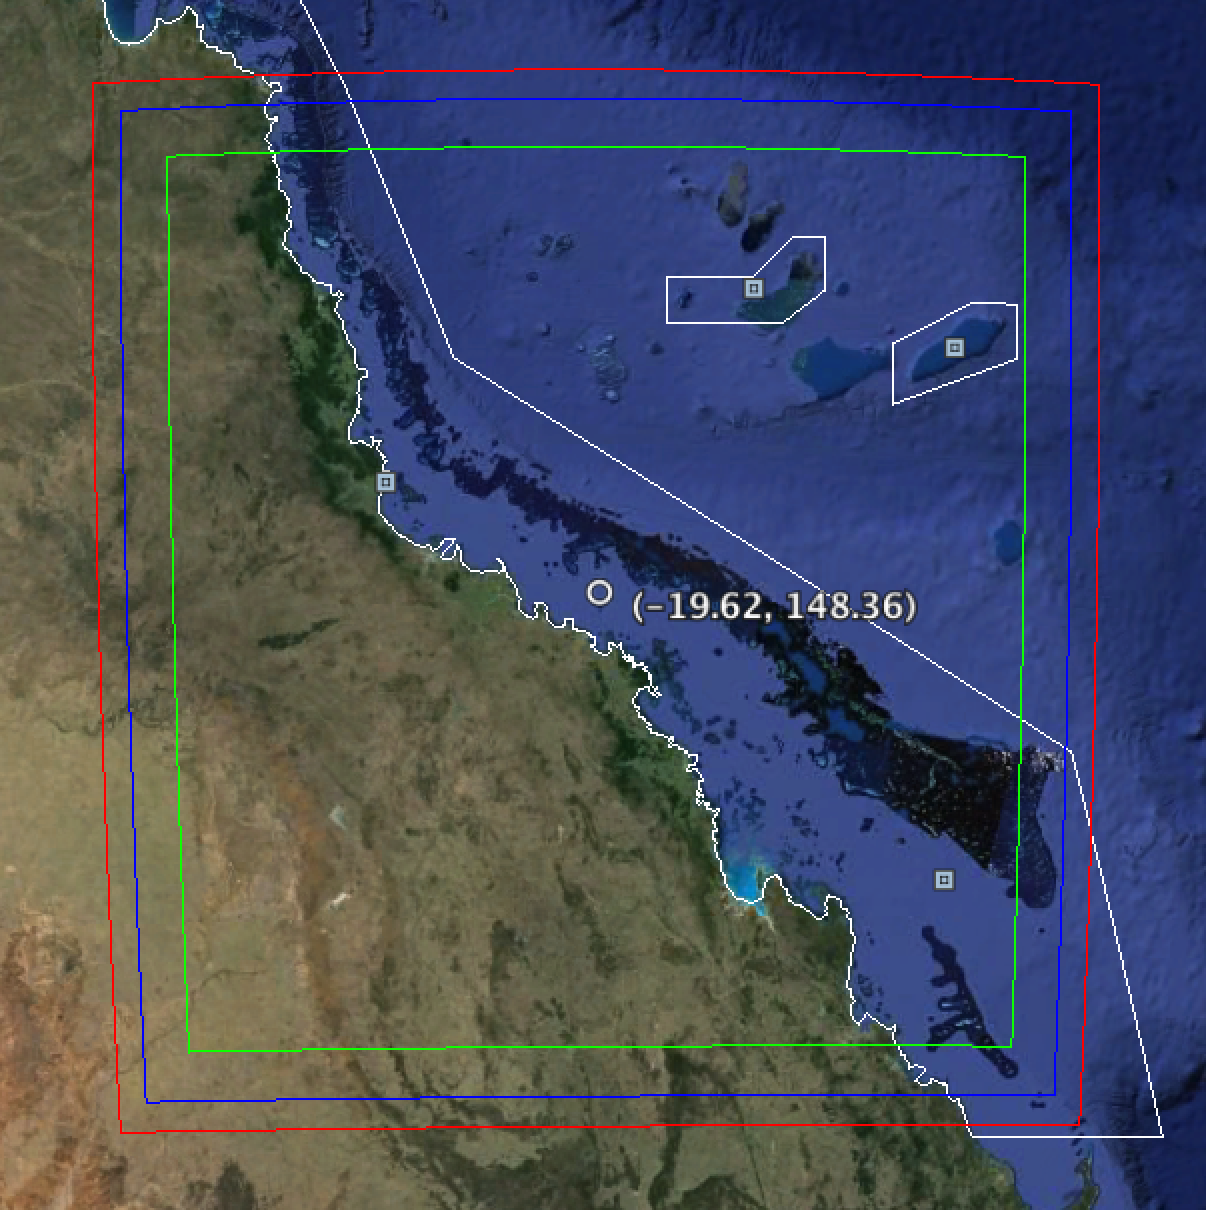
\includegraphics[width=0.6\textwidth,natwidth=1206,natheight=1210]{Fig/Research/EarthDomain.png}
    \caption{The final domain chosen (red) with its calculated \gls{ccam} (blue) and \gls{ctm} (green) domains overlaid onto the globe. The Great Barrier Reef Marine Park is shown in white.}
    \label{fig:earthdomain}
\end{figure}

The first domain, GBR 1, was chosen to capture long range effects within \gls{ccam} and \gls{ctm}. It encompasses the majority of Australia and out into the Pacific Ocean. The back trajectory modelling performed in the \gls{gbr} influenced the choice of the domains centre, and the size of the final domain. As seen in \cref{fig:btcoastoct}, the majority of the back trajectories come from the East and South-east. A location along the Queensland coast, with the greatest body of reef towards the East South-east of it, was chosen as the centre point (see \cref{fig:earthdomain}). The final domain GBR 3 includes both a portion of the Queensland coast-land, and the majority of the reef to the East South-east.

The \gls{ctm} domains were shrunk by \SI{10}{\percent} of the the \gls{ccam} domains, to avoid the singularities at the corners of the \gls{ccam} domains. There are other differences on top of this \SI{10}{\percent} margin that are a result of the way the domains had to be calculated for \gls{ccam} and \gls{ctm}. The equations illustrated in \cref{subsec:ctm} and \cref{subsec:ccam} were used for these domain calculations.

\subsection{Running the Models}
\label{subsec:runmodel}

The \gls{csiro} modelling systems required intensive computing power and so were run on \gls{csiro} operated super computers named Ruby and Pearcey. Ruby is supercomputer with a large number of nodes, but few cores per node and is mostly used for data manipulation and storage. Pearcey has a large number of cores per node and is used for running highly parallelised tasks. The first two \gls{ccam} domains were run on Ruby, as they were low enough resolution for the number of cores per node to matter less for run time. The queue for Ruby was substantially shorter than the queue for Pearcey. The final \gls{ccam} domain had to be run on Pearcey due to the high resolution. \gls{ctm} was run only on Ruby as the way in which it was parallelised couldn't take advantage of the high number of cores per node of Pearcey.  

To run \gls{ccam} a number of scripts had to be created to first set up the input data for the domains, and then to run the model itself. Care had to be taken to ensure the parameters used were compatible with \gls{ctm}. The same was true of \gls{ctm} however a larger number of scripts were used due to \gls{ctm} requiring more inputs such as fire sources, road sources and shipping sources. This is because \gls{ctm} simulates a large number of different chemicals and aerosol modes, requiring initial and boundary conditions. 

Due to the complexity, the \gls{ctm} runs ran into many problems and only a single day run was completed using the first two domains. This was even without some of the inputs such as shipping that would have been required to produce meaningful results. The preliminary run of \gls{ctm} for a single day was however enough to show that the \gls{ccam} runs had been performed correctly for use with \gls{ctm}.

\subsection{Comparison Data}
\label{subsec:domains}

To try and measure the accuracy of the output from \gls{ccam} measurement data was needed for comparison. The Australian Government's \gls{bom} collects such data and makes it available through its Climate Data Online tool \citep{bom}. The data is sorted by stations, of which there are hundreds all around Australia. Each station collects a number of different measurements such as temperature, wind speed, rainfall, humidity, pressure and so on. Not every station has the same measuring equipment and so some stations have no data for some measurements.

A number of station locations were selected to extract data from (see \cref{fig:bomlocsplot}). They were chosen for their location within the final \gls{ccam} domain (see \cref{fig:domains}) and for their locality along the coastline and within the \gls{gbr} as this was the region of focus. A script was written to extract the data in a form that was usable for comparison with the \gls{ccam} data.

\begin{table}[tbh!]
	\caption{\textsl{ The list of \gls{bom} locations that the \gls{ccam} output was compared to. }}
	\centering
		\begin{tabular}{c c c c} \\
			\hline 	\\ 	[-1ex]
			Station Number	&	Station Name	&	Latitude	&	Longitude	\\	[1ex]
			\hline	\\	[-1ex]						
			200283		&	Willis Island		&	-16.2878	&	149.9652	\\	
			031037		&	Low Isles			&	-16.3842	&	145.5592	\\	
			200879		&	Arlington Reef		&	-16.7226	&	146.1124	\\	
			200880		&	Lihou Reef			&	-17.133		&	152.145		\\	
			032141		&	Lucinda Point		&	-18.5203	&	146.3861	\\	
			033106		&	Hamilton Island		&	-20.3658	&	148.9536	\\	
			033119		&	Mackay				&	-21.1172	&	149.2169	\\	
			200001		&	Middle Percy Island	&	-21.6628	&	150.2711	\\	
			033294		&	Yeppoon				&	-23.1364	&	150.7506	\\	
			039122		&	Heron Island		&	-23.4417	&	151.9125	\\	
			039322		&	Rundle Island		&	-23.5293	&	151.2763	\\	
			039059		&	Lady Elliot Island	&	-24.1116	&	152.7161	\\	[1ex]
			\hline \\
		\end{tabular}
	\label{tab:bomlocs}
\end{table}

\begin{figure}[!htb]
    \centering
    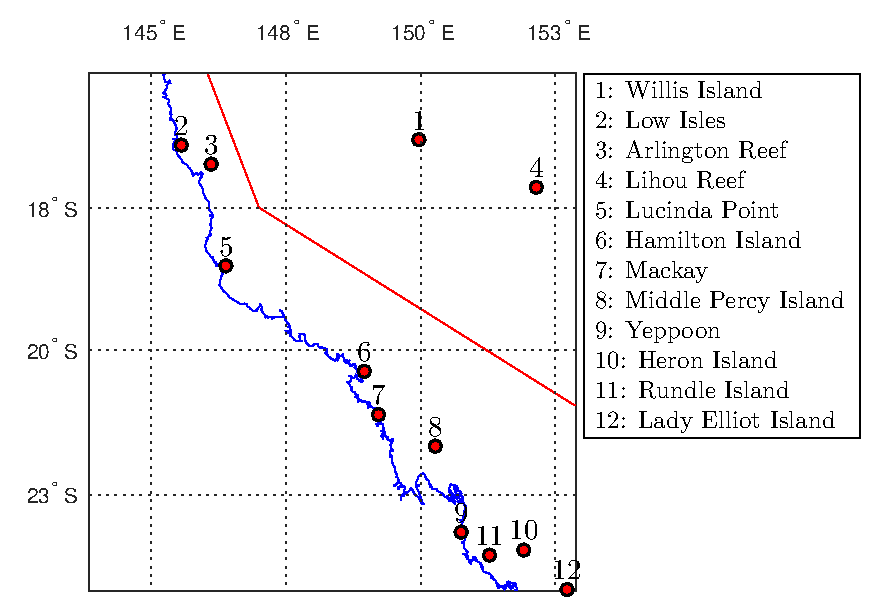
\includegraphics[width=0.9\textwidth]{Fig/Research/BomLocationsFinal2.eps}
    \caption{The locations of a number of \gls{bom} stations where data was taken from to compare with the results of the \gls{ccam} runs. }
    \label{fig:bomlocsplot}
\end{figure}

To quantify the difference between the measurements and model data two parameters were calculated. The first was the mean of the residuals $\bar{r}$. 
\begin{align}
	\label{eq:meanres}
	\bar{r} &= \frac{1}{n} \sum_{i=1}^n \left( c_i - b_i \right).
\end{align}
Where $n$ is the number of data points, generally $31$ for each day of October, and $b_i$ are the measurement data points collected from \gls{bom}. The \gls{ccam} data needed to be processed to extract a single value for each day, as the model output was hourly. Generally this took the form of finding the minimum or maximum value in the day to produce $b_i$. The mean residual provides direction and unit based scale of any differences.

The second quantifying parameter was the mean of percentage differences (\gls{mpd}) notated here as $\overline{PD}$.
\begin{align}
	\label{eq:meanpd}
	\overline{PD} &= \frac{1}{n} \sum_{i=1}^n \frac{\left| c_i - b_i \right|}{b_i}.
\end{align}
This uses the same variables as \cref{eq:meanres}. The \gls{mpd} uses the absolute value of the residuals to prevent cancellation if the individual residuals oscillate between positive and negative. It gives the magnitude of the difference, but normalised so that values from different sample locations can be compared. The standard deviation of the percentage differences was also calculated.

\subsection{CCAM Data Reduction}
\label{subsec:datared}

The variables output by \gls{ccam}, such as temperature or wind speed, are assembled as a 4D matrix. Two dimensions are the latitude and longitude, indicating location. The third is as series of pressure levels, which substitute for height as air pressure decreases vertically. The fourth dimension is time. Plotting \gls{ccam}'s output requires reduction of two of these dimensions.

To produce time series plots, the latitude and longitude dimensions need to be averaged. To do this either values across the entire map must be averaged, or a region of interest must be extracted at each time step and averaged. To create maps of the data, each latitude and longitude point can be averaged over time. Either way, the pressure levels also need to be averaged, or a single level must be selected. It is also possible to average over the spatial and time dimension and create a pressure level plot.

% maybe put a table of the different variables and their dimensions 

